% -*- root: ../../main.tex -*- %

There are several possibilities how Docker can be utilized for the execution of workflows.
Each combination of variants (abbreviated as depicted in Table~\ref{tab:docker_variants}) has its own advantages and disadvantages, which are elaborated in this chapter.

The first aspect is whether one wants to spread the containers associated with one workflow instance across various machines for execution ($S$) or constraint them to run on the same node as a group ($G$).

Second, one can differentiate to which extend workflow components are wrapped in their own containers.
One could encapsulate only activities in containers ($*_{AC}^{*}$) and distribute workflow information on another way, let each workflow and activity reside in a different container ($*_{SEPC}^{*}$), or wrap them in one container together ($*_{1C}^{*}$). Since this container is an atomic unit, it cannot be spread across many nodes for execution. One also could abandon the idea of a one-to-one mapping between the Docker and workflow concepts and establish worker containers with specialized behavior which perform suitable tasks on request ($*_{WORK}^{*}$).

Third, it is important to define the way data is exchanged between containers. One possible solution could be a data volume that is shared by all containers in need to exchange data with each other ($*_{*}^{DV}$). Data could also be passed between containers via some system service, \eg a database, ($*_{*}^{SER}$), or on a direct connection between the containers ($*_{*}^{D}$).

Finally, rather independent from the previous variants and hence discussed in isolation, one might want to choose the mechanism that decides which containers are run on which machines, \ie the execution scheduling.

\textcolor{red}{**TODO: table consistent with text?**}

\begin{table}[!htbp]
  \centering
  \begin{tabular}{C{4cm}|C{3cm}|C{3cm}|C{3cm}}
    \toprule
    \textbf{Data Exchange / Containerization}

    & Common Data~Volume  & Service & Direct \\ \midrule

    \multicolumn{4}{c}{\textbf{Grouped execution on one node} }\\ [1ex] \midrule

    Activities in containers
    & $G_{AC}^{DV}$   & $G_{AC}^{SER}$  & $G_{AC}^{D}$   \\ \midrule

    Workflows and activities in separate containers
    & $G_{SEPC}^{DV}$  & $G_{SEPC}^{SER}$ & $G_{SEPC}^{D}$  \\ \midrule

    Workflow and activities in one container
    & $G_{1C}^{DV}$  & $G_{1C}^{SER}$ & $G_{1C}^{D}$  \\ \midrule

    Worker containers
    & $G_{WORK}^{DV}$  & $G_{WORK}^{SER}$ & $G_{WORK}^{D}$  \\ \midrule

    \multicolumn{4}{c}{\textbf{Spread execution over available nodes} }\\ [1ex] \midrule

    Activities in containers
    & \xmark & $S_{AC}^{SER}$ & $S_{AC}^{D}$ \\ \midrule

    Workflows and activities in separate containers
    & \xmark & $S_{SEPC}^{SER}$ & $S_{SEPC}^{D}$ \\ \midrule

    Workflow and activities in one container
    & \xmark & \xmark & \xmark \\ \midrule

    Worker containers
    & \xmark & $S_{WORK}^{SER}$ & $S_{WORK}^{D}$ \\ \midrule

    \bottomrule
  \end{tabular}
  \caption{Containerization/Grouping/Communication Solution Pairings}
  \label{tab:docker_variants}
\end{table}

\subsection{Properties and mode of operation of the utilization variations} % (fold)
\label{sub:mode_of_operation_of_the_aspects}
\textcolor{red}{  **mehr einleitung hier**}
  In the following, the previously briefly introduced concepts are explained in more detail and some variations on them are given. Further, special interrelations among these traits are highlighted.

  \subsubsection{Grouped or spread execution} % (fold)
  \label{ssub:grouped_or_spread_execution}
    These variations are about the allocation of containers related to one workflow instance on the available nodes. While \ref{sub:execution_scheduling} deals with the mechanisms behind the scheduling, the larger concept of grouped or spread execution will be focused here.

    On the one hand, one could assign the containers to different nodes ($S_*^*$). This could happen at random, with regards to characteristics of the containers or their underlying workflow elements, or based on the current workload of the nodes. Balancing the workload and matching containers to specific nodes could have a positive impact on the performance of the execution. Negative effects might arise from the introduced network latency, though. Also, spread execution requires the images that belong to the workflow elements in question to be present on all nodes.

    On the other hand, the first container of a workflow enactment might be assigned to one node and all subsequently started containers are started on that same node ($G_*^*$). While this reduces the ability to balance the workload across nodes, it could be beneficial for the speed of communication between containers, since no transfer via network is required.
  % subsubsection grouped_or_spread_execution (end)

  \subsubsection{Element-wrapping Images} % (fold)
  \label{ssub:element_wrapping_containers}
    The general idea behind this set of concepts is that activities and workflows can be represented by images, activity instances and workflow instances by containers.

    As described in \ref{sec:concepts}, activities can be perceived as self-contained units of work, that is, they contain the information on how to autonomously perform a task on a given set of data.
    Analogously, Docker images contain the information on how to run processes in an instance of themselves -- a container -- given a set of parameters. If the work that an activity performs can be manifested in  program code, this code and its required runtime environment could be contained in a Docker image. An instance of that image that is created with a specific set of data would then be the counterpart of an activity instance. This notion is the foundation for the $*_{AC}^{*}$ and $*_{SEPC}^{*}$ variants.

    A similar train of thought can be applied to workflows: they contain the information that is necessary to perform sequences of tasks in an automated way. The sequence order is usually given in a formalized way by a process definition. In the given mindset, this process definition would be a list of Docker images in combination with a formal description of the control flow and data flow between these images. A workflow can thus be seen as a set of appropriate images and a corresponding process definition.
    A workflow instance, in turn, would consist of the relevant containers, the data that is used and created by these containers, and the enactment state of the workflow. These conceptual mappings are summarized in Figure~\ref{fig:conceptual_correspondence_between_wfms_and_docker_entities}.

    Like activities, workflows can thus be represented by images. Such a workflow image could contain the process definition of the respective workflow and other data that is specific to it. Alternatively, the workflow data may be passed to the workflow engine for enactment in another format.
    The variant in which the workflow information is distributed in a separate image along with the activity images is referred to in the following as $*_{SEPC}^{*}$, while the variant in which the workflow information is passed along otherwise is denoted as $*_{AC}^{*}$.
    Theoretically, a workflow could be completely encapsulated in an image, \ie with all its related activities and its configuration. This case is referred to as $*_{1C}^*$.

    \begin{figure}[htbp]
      \centering
        \begin{tabular}{r c l}
          \toprule
          Activity           & $\rightarrow$ & Image\\
          Activity instance  & $\rightarrow$ & Container\\
          Process definition & $\rightarrow$ & List of images + control flow + data flow\\
          Workflow           & $\rightarrow$ & Activity images + process definition\\
          Workflow instance  & $\rightarrow$ & Activity containers + data + enactment status\\
          \bottomrule
        \end{tabular}
      \caption{Possible Mapping of WfMS and Docker Concepts}
      \label{fig:conceptual_correspondence_between_wfms_and_docker_entities}
    \end{figure}

    Wrapping activities -- and optionally workflows -- in Docker images creates new possibilities in regard to their distribution and enactment. Images can be uploaded to public or private image registries to provide a standardized way for the deployment to nodes. This offers a way to make the deployment available as a service. Nodes can be instructed to contact these registries in order to be provided with required images or update existing ones.

    The layering principle behind Docker images makes updates to activity and workflow images lightweight -- as long as only the uppermost layers are changed, the lower ones do not have to be up- and downloaded again. This allows to distribute a complete runtime environment to new nodes while updating only specific layers on existing nodes using one and the same image.

    Containers can be paused and unpaused, \ie all processes within them are suspended. This is useful to save processor capacity for suspended activities or workflows until they are resumed.

    ** Second, $*_{*}^{SEPC}$ leverages the already existing communication between a container, the local daemon and the swarm master to communicate the status of workflow instances and activity instances, as the creation of a container

    **more benefits here**


    \begin{figure}[htbp]
      \centering
      \begin{tikzpicture}[->,>=stealth',shorten >=1pt,auto,node distance=5cm, semithick]
        \sffamily\fontsize{10}{10}\selectfont
        \node (cr){};
        \node (run){};
        \node[state] (A)     [right =3cm of cr]         {created};
        \node[state]         (B) [right =2.5cm of A] {running};
        \node[state]         (C) [below right of=B] {stopped};
        \node[state]         (D) [above =2cm of B] {paused};
        \node[state]         (E) [below of=A] {deleted};

        \path (cr) edge [] node {create} (A)
            (run) edge [out=45,in=150]                     node {run} (B)
              (A) edge []                              node {start} (B)
                  edge [bend right]                    node {rm}    (E)
              (B) edge [out=230, in=200, distance=4cm] node {kill}  (C)
                  edge [out=250,in=175, distance=2.5cm]node {stop}  (C)
                  edge [bend left]                     node {pause}  (D)
                  edge [in=30, out=45, loop]           node {restart}  (D)
                  edge [out=10, in=90, distance=2cm]   node {\textit{container process exited}}  (C)
              (C) edge [bend right]                    node {start}  (B)
                  edge [bend left]                     node {rm}  (E)
              (D) edge [bend left]                     node {unpause} (B)
              ;
      \end{tikzpicture}
      \caption*{Simplified version. Commands should be understood prefixed with \textit{docker}. \newline \scriptsize Based on https://docs.docker.com/engine/reference/api/docker\_remote\_api/\#docker-events }
      \caption[Docker Container Life Cycle]{Docker Container Life Cycle \cite{Docker2016Docker}}
      \label{fig:docker_container_lifecycle}
    \end{figure}

    One possible variation on $G_{1C}^{DV}$ and $G_{SEPC}^{DV}$ would be the inclusion of engine logic in the workflow instance container. While the scheduling of this container and preparations on the targeted node would still be in the responsiblity of the main \acp{WfMS}' workflow engine, the control over the started activity instances would be handed to a smaller, workflow instance specific engine.
    This setup facilitates the management of the required directory structure, since the container that issues the commands has direct access to the data volume -- no information on the upcoming element instances has to be transferred.

    Further, in this case suspending and resuming of workflows and activities could both be realized with the respective pause/unpause Docker commands. In combination with a checkpoint/restore tool, which provides the means to save and restore the memory state of a process, long running workflows could be paused and restored across server restarts, or be migrated to another server, if necessary. Proofs of concept for the feasibility of this procedure have been presented in the past \cite{Kim2015Checkpoint,Merker2015How}.

    A drawback of this variation is, that the status of the enactment is then held in the workflow instance container. By following the event stream, started and stopped activity instances could be tracked by the main workflow engine, but low-level details would have to be transferred separately, if it was needed there.
  % subsubsection element_wrapping_containers (end)

  \subsubsection{Worker Containers} % (fold)
  \label{ssub:worker_containers}
    The $*_{WORK}^{*}$ variants take a different approach at utilizing Docker for workflow enactment, in which many unspecialized containers are running constantly. These containers, when provided with an activity description and input data, perform the required actions and return to a waiting state until they are provided with a task again.

    Opposed to the variant presented in \ref{ssub:element_wrapping_containers}, there is no one-to-one correlation of an image to an activity or a workflow, and also none of a container to an activity instance or a workflow instance. Hence, there is no further creation and distribution of images required -- besides the initial distribution of the workers' images (and, eventually, invoked third-party images).
    Since all information that is required for execution is passed to these workers at each invocation, changes to definitions of activities or workflows may immediately show effects. This flexibility comes at the price of a verbose communication, though.

    Another benefit of worker containers is that they facilitate swift adaption to workload peaks. In case that scheduled enactments start to accumulate, more worker containers may be run. If the nodes themselves have reached their resource limitations, new nodes may be added to the swarm, which do not have to be provisioned with all activity or workflow images -- as it would be the case with the wrapping-images variant -- but rather only with the worker image.
  % subsubsection worker_containers (end)

  \subsubsection{Data Exchange via Data Volume} % (fold)
  \label{ssub:data_exchange_via_data_volume}
    The idea behind this concept ($*_{*}^{DV}$) is, that all containers involved in the execution of one workflow instance have access to a common working directory, in which the data visibility scopes can be established using a file system structure. This working directory resides in a data volume owned by a container that belongs exclusively to the respective workflow instance and whose only purpose is to ensure the existence of said volume.

    % - data volume mountable via -v option
    % - arbitrary name and location in container

    In its simplest form the working directory could be a simple shared directory, which is managed cooperatively by all related containers. Activity instances could then read and write files to that directory.
    \textcolor{red}{**PRO/CON?**}

    A more elaborate structure could be imposed on the working directory, too. In order to support the data visibility and data interaction types that were chosen in \ref{ssub:workflow_execution}, the following directory structure could be used, which is depicted in Figure~\ref{fig:dv_dir_structure}.
    Data defined at build time, \ie environment data, workflow data and activity data, could each be stored in a separate subdirectory of the main working directory \texttt{workflow\_relevant\_data}. The directories for workflow data and activity data should have uniquely identifyiable names that can be infered from the respective workflow element, \eg \texttt{wf\_\$workflow\_id} and \texttt{ac\_\$activity\_id}. Data that is shared among multiple instances of one activity could be stored in a subdirectory \texttt{shared} of the respective activity data directory.

    Also present in the working directory should be a directory \texttt{wfi\_\$workflow\_instance\_id}, in which the working directories for subsequently started activity instances and workflow instances can be stored. Each activity instance is then assigned a directory \texttt{aci\_\$activity\\\_instance\_id} within that that working directory. In case that the activity instance in question is a sub-workflow activity, the respective workflow instance's working directory resides in the sub-workflow activity instance's working directory. This principle can then be repeated recursively, as visible in Figure~\ref{fig:dv_dir_structure}.

    Depending on the desired level of isolation, the instance containers could be instructed to mount either a) the whole \texttt{workflow\_relevant\_data} directory or b) just their own working directory, the directories that contain the data defined at build time, and working directories of activity or workflow instances which they were configured to use. While the former is a much simpler solution, the latter gives more fine-grained control over the data that each instance is allowed to access.

    \begin{figure}[htbp]
      \centering
      \begin{forest}
        dir tree
        [workflow\_relevant\_data
          [env]
          [wf\_1cc594ba-...]
          [wf\_b45d2564-...]
          [ac\_0225d86f-...
            [shared]
          ]
          [ac\_2a5aa4ff-...]
          [ac\_7fc09132-...]
          [wfi\_e65c8533-... \textcolor{gray}{(instance of wf\_1cc594ba-...)}
            [aci\_76b8680c-... \textcolor{gray}{(instance of ac\_0225d86f-...)}]
            [aci\_1e09d287-... \textcolor{gray}{(instance of ac\_2a5aa4ff-...)}
              [wfi\_68e17268-... \textcolor{gray}{(instance of wf\_b45d2564-...)}
                [aci\_2708fd1a-... \textcolor{gray}{(instance of ac\_7fc09132-...)}]
              ]
            ]
          ]
        ]
      \end{forest}
      \caption{Exemplary directory structure for $G_{*}^{DV}$}
      \label{fig:dv_dir_structure}
    \end{figure}


    $G_{*}^{DV}$ natively supports all identified types of data visibility by providing respective directories and access to them, with the limitation that workflow data and environment data has to be copied to the data volume before execution and is thus restricted to the state it had at that time. Altering this data is possible, \eg by replacing the respective files via \texttt{docker copy} or altering it in a \texttt{docker exec} session, but extra measures have to be taken to request such an up-to-date version.

    Data interactions between activity instances, a sub-workflow activity and its related components and vice versa are supported by $G_{*}^{DV}$. Exchanging data between two running workflow instances is not possible on this way, since mounting volumes to running containers is not supported by Docker yet. This kind of interaction thus requires some additional tools. It would be possible to grant access to workflow instances running on the same machine -- at the price of loss of control over data visibility -- by mounting the top-level working directory of that machine in all containers.

    As long as no requests to external sources are made within the workflow, data has to be transferred over the network only twice in this approach -- for the input and output of the workflow instance. All subsequent data transfers are either implicit, \eg by accessing the respective working directory or a symbolic link to it, or take place on the local machine, \eg copying one or more files. Because of transfer rates *QUOTE*, $G_{*}^{DV}$ has an advantage over message-based approaches when it comes to processing of large and/or many data sets, \ie log files, genome research data or images. Also, unless required by the activities themselves, data conversion is less of an issue since relying on the file system allows arbitrary file types to be used.

    Sharing a data volume using only Docker tools requires all containers to be on the same machine, which is why there is no spread version $S_{*}^{DV}$ of this concept. Approaches exist to utilize \ac{NFS} or \ac{P2P} file sharing for distributed access to data volumes, but given the limited scope of this thesis they shall not be regarded further here \cite{Miell2015How}.

    $G_{1C}^{DV}$ could theoretically work on its own file system in the editable layer of the container without a dedicated data volume, since all workflow components would have access to it. This would make the container self contained on the one hand -- and thus easier to export or migrate -- but would on the other hand couple the data life cycle to the processing container's life cycle. That is, if the container is removed, the data is removed with it.

    In order for $G_{WORK}^{DV}$ to work successfully, it is inevitable that only workers on the same node as the data volume are used for the workflow enactment, since workers on different nodes could not access that data volume.
  % subsubsection data_exchange_via_data_volume (end)

  \subsubsection{Data Exchange via Service} % (fold)
  \label{ssub:data_exchange_via_service}
    $*_{*}^{SER}$ represents the concept of providing some service that is able to store and serve workflow relevant data on request. This implies, that the instance containers have to feature a mechanism to communicate to this service.

    The data-providing service could either be running as a single instance on some node in the network or on each node in the network. While the former avoids having to deal with synchronization between service instances and inconsistencies resulting from race conditions, the latter could balance the load. (shorten response times? hops)

    Since the storage of workflow related data is decoupled from the execution in $*_{*}^{SER}$, the coverage of data visibility and data interaction capabilities depends on the chosen underlying service. Theoretically, all forms of data visibility and interactions should thus be possible. Also, the solution exhibits the same properties for grouped and spread execution alike, for the same reason.

    In this variant, data is transferred before and after each step in the workflow, \ie when the execution starts, when it ends, whenever an activity is instantiated or an instance finished its work. This is only economical if the amount of data is sufficiently small or if the workflows consist of few activities. In order for the workflow execution to function correctly, the data management service must be reliably available to all containers.
  % subsubsection data_exchange_via_service (end)

  \subsubsection{Data Exchange via Direct Communication} % (fold)
  \label{ssub:data_exchange_via_direct_communication}
    In this scenario, the containers communicate with each other directly in order to exchange workflow relevant data. It can be split again in two sub-variants, according to the data passing patterns noted in \ref{sub:workflow_data}. On the one hand, one where the workflow relevant data is passed along the control flow ($*_{*}^{D_a}$). On the other hand, one where containers can query each other for their data($*_{*}^{D_b}$).

    In $*_{*}^{D_a}$, the data flow is is directly coupled to the control flow, \ie all data is passed on on invocation. This requires all data that might be used in another activity instance to be passed along, no matter whether the succeeding activity uses them or not \cite{Russell2005Workflow}. While this variant allows to pass (and update) workflow and environment data, it may be problematic for larger amounts of data.

    $*_{*}^{D_b}$ requires all containers that shall be queried for data to provide some communication mechanism and to be running. Thus, in the worst case every container related to the workflow instance in question has to be kept running. Even though the containers' use of processor time can be reduced by pausing them until they are needed, this approach could impose a considerable strain on the host machine's memory, as pausing containers has no effect on their memory consumption.
    Workflow data and environment data in $*_{*}^{D_b}$ may be provided to the first activity, which then could be queried for a (static) version of it.

    Because workflow instances are not represented as containers in $*_{AC}^{D}$, $*_{AC}^{D_b}$ provides no means to store and access sub-workflow data, multiple instance data and workflow instance data.

    $*_{WORK}^{D_b}$ is no useful solution, as keeping the worker containers occupied with one activity in order to make them queryable would block their use for other workflow instances, thus rendering the \ac{WfMS} incapable of processing further workflow instances once all workers are invoked -- unless further workers are spawned.

    As all workflow components reside in one container in $G_{1C}^{D}$, no communication between containers is necessary -- all data can be exchanged on an arbitrary way within that single container. This variant thus represents a special case.
  % subsubsection data_exchange_via_direct_communication (end)
% subsection mode_of_operation_of_the_aspects (end)

\begin{table}[!htbp]
  \centering
  %\renewcommand*{\arraystretch}{1.7}
  \begin{tabular}{C{1cm} C{1cm} C{1cm} C{1cm} C{1cm} C{1cm} C{1cm} | C{1cm} C{1cm} C{1cm} C{1cm}}
    \toprule

    \multicolumn{6}{c}{Data Visibility} & \multicolumn{4}{c}{Data Interactions} \\

      & \rot{Ac Data}
      & \rot{SubWF Ac Data}
      & \rot{MultInst Ac Data}
      & \rot{WFInst Data}
      & \rot{WF Data}
      & \rot{Env Data}

      & \rot{Ac $\rightarrow$ Ac}
      & \rot{SubWF Ac $\rightarrow$ SubWF}
      & \rot{SubWF $\rightarrow$ SubWF Ac}
      & \rot{WFInst $\rightarrow$ WFInst}
    \\ \midrule

    $G_{AC}^{DV}$    & \ja     & \ja              & \ja              & \ja              & \ja ($\dagger$) & \ja ($\dagger$) & \ja              & \ja              & \ja              & $\bigcirc$      \\ \midrule
    $G_{SEPC}^{DV}$  & \ja     & \ja              & \ja              & \ja              & \ja ($\dagger$) & \ja ($\dagger$) & \ja              & \ja              & \ja              & $\bigcirc$      \\ \midrule
    $G_{1C}^{DV}$    & \ja     & \ja              & \ja              & \ja              & \ja ($\dagger$) & \ja ($\dagger$) & \ja              & \ja              & \ja              & $\bigcirc$      \\ \midrule
    $G_{WORK}^{DV}$  & \ja     & \ja              & \ja              & \ja              & \ja ($\dagger$) & \ja ($\dagger$) & \ja              & \ja              & \ja              & $\bigcirc$      \\ \midrule

    $G_{AC}^{SER}$   & \ja     & \ja              & \ja              & \ja              & \ja             & \ja             & \ja              & \ja              & \ja              & \ja             \\ \midrule
    $G_{SEPC}^{SER}$ & \ja     & \ja              & \ja              & \ja              & \ja             & \ja             & \ja              & \ja              & \ja              & \ja             \\ \midrule
    $G_{1C}^{SER}$   & \ja     & \ja              & \ja              & \ja              & \ja             & \ja             & \ja              & \ja              & \ja              & \ja             \\ \midrule
    $G_{WORK}^{SER}$ & \ja     & \ja              & \ja              & \ja              & \ja             & \ja             & \ja              & \ja              & \ja              & \ja             \\ \midrule

    $G_{AC}^{D_a}$   & \ja     & \ja              & $\bigcirc$       & \ja              & \ja             & \ja             & \ja ($\ddagger$) & $\bigcirc$       & $\bigcirc$       & $\bigcirc$      \\ \midrule
    $G_{AC}^{D_b}$   & \ja     & $\bigcirc$       & $\bigcirc$       & $\bigcirc$       & $\bigcirc$      & $\bigcirc$      & \ja ($\ddagger$) & $\bigcirc$       & $\bigcirc$       & $\bigcirc$      \\ \midrule
    $G_{SEPC}^{D}$   & \ja     & \ja ($\ddagger$) & \ja ($\ddagger$) & \ja ($\ddagger$) & $\bigcirc$      & $\bigcirc$      & \ja ($\ddagger$) & \ja ($\ddagger$) & \ja ($\ddagger$) & \ja ($\ddagger$)\\ \midrule
    $G_{1C}^{D}$     & \ja$^*$ & \ja$^*$          & \ja$^*$          & \ja$^*$          & $\bigcirc$      & $\bigcirc$      & \ja$^*$          & \ja$^*$          & \ja$^*$          & \ja$^*$         \\ \midrule
    $G_{WORK}^{D}$   & \ja     & \ja ($\ddagger$) & \ja ($\ddagger$) & \ja ($\ddagger$) & $\bigcirc$      & $\bigcirc$      & \ja ($\ddagger$) & \ja ($\ddagger$) & \ja ($\ddagger$) & \ja ($\ddagger$)\\ \midrule

    $S_{AC}^{SER}$   & \ja     & \ja              & \ja              & \ja              & \ja             & \ja             & \ja              & \ja              & \ja              & \ja             \\ \midrule
    $S_{SEPC}^{SER}$ & \ja     & \ja              & \ja              & \ja              & \ja             & \ja             & \ja              & \ja              & \ja              & \ja             \\ \midrule
    $S_{WORK}^{SER}$ & \ja     & \ja              & \ja              & \ja              & \ja             & \ja             & \ja              & \ja              & \ja              & \ja             \\ \midrule

    $S_{AC}^{D}$     & \ja     & $\bigcirc$       & $\bigcirc$       &  $\bigcirc$      & $\bigcirc$ & $\bigcirc$  & \ja ($\ddagger$) & $\bigcirc$       & $\bigcirc$       & $\bigcirc$      \\ \midrule
    $S_{SEPC}^{D}$   & \ja     & \ja              & \ja              & \ja              & $\bigcirc$ & $\bigcirc$  & \ja ($\ddagger$) &\ja ($\ddagger$)  & \ja ($\ddagger$) &\ja ($\ddagger$) \\ \midrule
    $S_{WORK}^{D}$   & \ja     & \ja              & \ja              & \ja              & $\bigcirc$ & $\bigcirc$  & \ja ($\ddagger$) &\ja ($\ddagger$)  & \ja ($\ddagger$) &\ja ($\ddagger$) \\ \bottomrule
  \end{tabular}
  \captionsetup{justification=centering}
  \caption*{\ja~ natively supported ~~|~~ \ja$^*$~ natively supported, a direct connection within the container is assumed ~~|~~ \ja ($\dagger$)~ can be passsed on instantiation, real-time access requires additional tools \\ \ja ($\ddagger$) natively supported, assuming that all containers are left running for the time of workflow execution ~~|~~ $\bigcirc$~ not natively supported, requires additional tools \\[1em]

  Ac = Activity ~|~ SubWF = Sub-workflow~|~ MultInst = Multiple instance ~|~ WFInst = Workflow instance~|~ WF = Workflow ~|~ Env = Environment
  }
  \label{tab:docker_variants}
  \caption{Containerization/Grouping/Communication Solution Pairings}
\end{table}

\subsection{Identification of promising combinations} % (fold)
\label{sub:promising_combinations_of_characteristics}
  Due to its shortcomings regarding the supported types of data visibility and interactions, direct communication between instance-related containers ($*_{*}^{D}$) is ruled out as a candidate for the prototype. The remaining combinations may be eligible depending on the intended use case and desired properties of the \ac{WfMS}, \eg the kind of data that is processed, the targeted infrastructure, and nature of the workflows.

  If the data volume approach is chosen, one is committed to grouped execution on one node. Considering the different containerization solutions, $G_{SEPC}^{DV}$ is favorable over $G_{AC}^{DV}$, because the explicit existence of containers which represent (sub-)workflow instances makes it possible to both track their state using Docker mechanisms and manage their respective working directories. Embedding workflow engine logic into these containers could enable workflows to be exported and used in a stand-alone fashion.

  $G_{SEPC}^{DV}$ is also favorable over $G_{1C}^{DV}$ for general use, because the modularity of $G_{SEPC}^{DV}$ permits to update single activities within the workflow by distributing new versions of their respective image. In $G_{1C}^{DV}$, the whole image would have to be updated due to the way layering in Docker images works. Also, $G_{1C}^{DV}$ does not provide the means to track the activity instances' life cycles with Docker mechanisms, only that of the workflow instance. If the workflow is not meant to be updated but to be distributed to third parties as a stand-alone solution, \eg an automated batch process for photos, which is sold to photographers, this variant could be a viable option, however.

  The main benefit of $*_{WORK}^{*}$ is that it allows to distribute the workload among several workers. Since $G_{*}^{DV}$ requires all involved workers to be on the same machine, this advantage is void for the combination $G_{WORK}^{DV}$.

  Altogether, this makes $G_{SEPC}^{DV}$ the variant of choice for data-intense use cases.

  When comparing the service-based variants with each other, $G_{*}^{SER}$ and $S_{*}^{SER}$ share most their advantages and drawbacks. $S_{*}^{SER}$ permits the containers to run on different nodes, though. As this allows containers to be assigned to machines according to their resource requirements and the momentary workload of a machine, it is the preferred variant of those two.

  Because the decoupling of data and containers is well supported by $*_{*}^{SER}$, it is a good fit for the worker-based approach of $*_{WORK}^{*}$, which in turn facilitates load balancing. A use case for $S_{WORK}^{SER}$ could be \ac{WfMS} users like market research companies, which create lots of frequently updated form-centric workflows for call center agents to use, \ie fast-changing workflows with rather small data that has to be passed.

  The results of the above reasoning are roughly summarized in a decision tree in Figure~\ref{fig:choosing_docker_utilization}, which is intended to give a hint on the suitable utilization of Docker for workflow enactment for a given use case.

  \begin{figure}[htbp]
    \centering
    \newdimen\nodeDist
    \nodeDist=35mm
    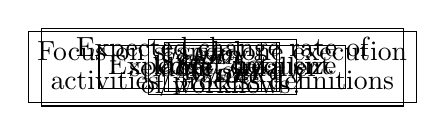
\begin{tikzpicture}[
        node/.style={%
          draw,
          rectangle,
        },
      ]

        \node [align=center, node] (A) {Focus on standalone execution \\of workflows?};
        \path (A) ++(-135:\nodeDist) node [align=center, node] (B) {$G_{1C}^{DV}$};
        \path (A) ++(-45:\nodeDist) node [align=center, node] (C) {Expected data size};
        \path (C) ++(-135:\nodeDist) node [align=center, node] (D) {$G_{SEPC}^{DV}$};
        \path (C) ++(-45:\nodeDist) node [align=center, node] (E) {Expected change rate of \\ activities/process definitions};
        \path (E) ++(-45:\nodeDist) node [align=center, node] (F) {$S_{WORK}^{SER}$};
        \path (E) ++(-135:\nodeDist) node [align=center, node] (G) {$S_{AC/SEPC}^{SER}$};

        \draw (A) -- (B) node [left,pos=0.5] {yes}(A);
        \draw (A) -- (C) node [right,pos=0.5] {no}(A);
        \draw (C) -- (D) node [left,pos=0.5] {large}(A);
        \draw (C) -- (E) node [right,pos=0.5] {smaller}(A);
        \draw (E) -- (F) node [right,pos=0.5] {frequent}(A);
        \draw (E) -- (G) node [left,pos=0.5] {seldom}(A);
    \end{tikzpicture}
    \caption{Choosing the right utilization of Docker for workflow enactment}
    \label{fig:choosing_docker_utilization}
  \end{figure}
% subsection promising_combinations_of_characteristics (end)

\subsection{Utilization of third-party images} % (fold)
\label{sub:execution_of_third_party_containers}
  The motivation behind enabling the use of third-party images is that theoretically, any program which is able to run in a Docker container may be incorporated in a workflow this way. In 2015, over 125.000 public repositories existed \cite{Dehamer2015Docker}.

  Before these images can be used by a workflow instance, they have to be present on the node that they will be run on. The provision of nodes with the required images could either happen actively, thus qualifying the node for the execution of said image, or passively, \ie the node is selected for running the image in question and fetches it in the course of running it. While the the former solution limits the number of nodes that are able to run the image -- unless every node is provisioned with it -- the latter solution is likely to delay the enactment of the workflow at its first use for the time it takes to pull the respective image.

  As third-party images are likely to be unaware of their utilization in a workflow, it is not guaranteed that their output suits the needs of the \ac{WfMS}. Also, these images may require some parametrization for their instantiation. On the one hand, both issues could be approached by the workflow engine, which might transform the output and provide suitable parameters based on the activity's configuration. On the other hand, an utility activity could be introduced that can be configured such that it is able to instantiate the third-party image and transform its output to a suitable format.
  The latter solution should be preferred, as it shifts the responsibility for the aforementioned tasks away from the workflow engine, which reduces the engine's complexity. The engine does not need to differentiate between custom and foreign images in this case.

  \textcolor{red}{**Argumentation schwach**}

  In order to be able to instantiate the third-party image, the adapter image requires access to its host node's Docker daemon.
% subsection execution_of_third_party_containers (end)


\subsection{Execution Scheduling} % (fold)
\label{sub:execution_scheduling}
  In the course of a workflow enactment, several containers have to be instantiated -- unless the worker-based approach ($*_{WORK}^{*}$) is chosen. Choosing the node on which the instantiation takes place is a task that may impact the performance of the containers and the enactment itself, as the nodes may differ regarding their available resources. It is thus of interest to examine by which rules or criteria the scheduling may take place and whether and how the user should be able to take influence on the scheduling.

  \subsubsection{Scheduling Abilities of Docker Swarm} % (fold)
    \label{ssub:abilities_of_docker_swarm}
    As mentioned in \ref{sub:docker_swarm}, Docker Swarm offers two kinds of scheduling mechanisms: filters and strategies. Filters can be passed on instantiation as an environment variable parameter with the format \texttt{<filter-type>:<key><operator><value>}. The value of \texttt{filter-type} can either be ``constraint'' or ``affinity'' -- the two types of filters supported by Swarm.

    \texttt{<key>} can take the values \emph{node} or \emph{container} (which signals a comparison to the respective name or \ac{ID}), one of the default node tags, or the name of some custom label which can refer to both node labels and container labels. By default, nodes get tagged by Docker with a name, their \ac{ID}, their storage driver, their execution driver, the kernel version they use and the name of their operating system.
    Custom labels may be applied to nodes when their daemon is started and to containers as a parameter to the \texttt{run} command. In order to avoid conflicting label names, reverse domain name notation is advised by Docker.
    \texttt{<operator>} may either take the value \texttt{==} or \texttt{!=}, indicating whether a match is desired or should be avoided. It can be followed by a tilde, \eg \texttt{==~} to signal that if the condition cannot be met, the container should be scheduled according to a strategy instead.
    The \texttt{<value>} is a string made of alpha-numeric characters, dots, hyphens, and underscores. It may be either a regular expression or a globbing pattern, to which names, \acp{ID} tags or labels will be matched against.

    Constraints focus on the characteristics of nodes for scheduling; either \ref{itm:const_first} some identifier or \ref{itm:const_second} node tags or \ref{itm:const_third} labels:

    \begin{enumerate}[label=\alph*), nosep]
      \item \label{itm:const_first} \texttt{constraint:node==...}
      \item \label{itm:const_second} \texttt{constraint:operatingsystem==...}
      \item \label{itm:const_third} \texttt{constraint:com.example.label==...}
    \end{enumerate}

    Affinities can be specified to schedule containers based on the presence of images or containers on the target node. Possible criteria are \ref{itm:aff_first} container names or \acp{ID}, \ref{itm:aff_second} image names or \acp{ID} or \ref{itm:aff_third} a custom label on a container:

    \begin{enumerate}[label=\alph*), nosep]
      \item \label{itm:aff_first} \texttt{affinity:container==...}
      \item \label{itm:aff_second} \texttt{affinity:image==...}
      \item \label{itm:aff_third} \texttt{affinity:com.example.label==...}
    \end{enumerate}

    Further, there are some implicit forms of scheduling. First, containers will not be executed on nodes that Swarm considers \emph{unhealthy}, \ie that do not respond or otherwise exhibit faulty behavior. Second, some Docker features imply scheduling rules. If the container requires an exposed port, it will not be scheduled on nodes where this port is already occupied. Mounted volumes of, a shared network stack with or a link to another container imply an affinity to that container, which will prohibit the execution if it is not met.
  % subsubsection abilities_of_docker_swarm (end)

  \subsubsection{Identification of Possible Scheduling Criteria} % (fold)
  \label{ssub:identification_of_desired_scheduling_criteria}
    In order to examine scheduling solutions, some goals should be specified to which they can be evaluated against -- an exhaustive list of these goals is not in the scope of this thesis, though. Thus, two groups of exemplary scheduling criteria are considered, which are depicted in Table~\ref{tab:scheduling_criteria}.

    On the one hand, scheduling may be performed based on the properties of the nodes, which can be of qualitative or quantitative nature, their tags or the execution environment they have to offer. Examples for qualitative node properties could be its name, present containers or images, geographical location, the nature of its storage device, or its membership in some arbitrary groups. Quantitative properties of interest might be the amount of available memory or storage, the number of currently running containers or the node's network speed.

    On the other hand, containers may be assigned to nodes based on \ac{WfMS}-specific data. This could be for example properties of the underlying activities and workflows, the status and data of their instances or the state of a custom scheduling mechanism of the \ac{WfMS}. For example, if a user specifies his/her current location in the course of a workflow enactment, all subsequent containers could be scheduled to run on nodes that suit the laws of that country.

    \begin{table}[!htbp]
      \centering
      \begin{tabular}{l l l}
        \toprule
        Data Source & Criterion Type & Examples \\
        \midrule
        Docker
          & Node tags
            & Name \\
            && \ac{ID} \\
            && Storage driver \\
            && Execution driver \\
            && Kernel version  \\
            && Operating system \\ [1.2ex]
          & Qualitative node properties
            & Geographic location\\
            && Custom grouping membership\\
            && Ownership status\\ [1.2ex]
          & Quantitative node properties
            & Available memory \\
            && Available storage \\
            && Network speed \\ [1.2ex]
          & Execution environment
            & Existing containers \\
            && Existing images \\
            && Currently running containers \\ [1.4ex]
        WfMS
          & Live data
            & Enactment status \\
            & Activity input/output data \\
            && Workflow input/output data \\ [1.2ex]
          & Activity/workflow properties
            & Expected data-intensity \\
            && Compliance requirements\\
            &&\\ [1.2ex]
        \bottomrule
      \end{tabular}
      \label{tab:scheduling_criteria}
      \caption{Scheduling Criteria}
    \end{table}

    Both qualitative and quantitative properties of a node can be stored in custom labels on that node.
    Qualitative values can simply be stored as strings and used in constraints via globbing and regular expressions. Assuming, for example, the nodes had their location stored as a label with the format

    \centerline{\texttt{com.example.location=\$country}}

    with \texttt{\$country} being the respective ISO 3166-1 alpha-2 code \cite{Standardization2013De}; and the information whether they belong to the own company or are rented servers stored as a label with the format

    \centerline{\texttt{com.example.internal=\$internal}}

    with \texttt{\$internal} being the string representation of a boolean value. Then, in order to schedule a container to a self-owned node in Germany running any version of the \emph{Ubuntu} operating system, the following combination of tag and label constraints could be used:

    \centerline{\texttt{constraint:operatingsystem==Ubuntu*}}
    \centerline{\texttt{constraint:com.example.location==de}}
    \centerline{\texttt{constraint:com.example.internal==true}}

    Quantitative values stored in a label may be queried with comparisons using regular expressions. Assuming all nodes have a label that specifies their amount of memory, which has the form

    \centerline{\texttt{com.example.ram=\$mem}}

    with \texttt{\$mem} being the amount of memory in megabytes. In this setting, a container can be scheduled to a node with at least 650 megabytes of memory by enforcing the constraint

    \centerline{\texttt{constraint:com.example.ram==/({\textbackslash}d{\textbackslash}d{\textbackslash}d{\textbackslash}d+|[7-9]{\textbackslash}d{\textbackslash}d|[6][5-9]{\textbackslash}d)/}}

    This regular expression will match a) any number with four or more digits and b) any three digits number that starts with a number in the range of 7-9 and c) any three digits number that starts with 6 and continues with a number in the range of 5-9. Analogously to this, other quantitative measures may be stored and queried.

    Scheduling constraints regarding present images and containers can be realized using the appropriate affinity filters. One possible use case is to ensure, that all images and containers required for the enactment of a workflow element are present:

    \centerline{\texttt{affinity:image==required-image-name}}
    \centerline{\texttt{affinity:container==required-container-name}}

    At the current state of Docker Swarm, it is not possible to make sure that the containers are not only present but also running. If it is required, this criterion has to be addressed by some custom mechanism of the \ac{WfMS}, \eg a method that queries the swarm master's \ac{API}, selects a suitable node with running instances of the required container and constructs an according node constraint.

    Since updating labels and tags of containers and nodes after their creation is not possible at the time of writing, all \ac{WfMS} related data created during enactment has to be sent to the system and managed internally by it.

    Properties of activities and workflows that has been defined at build time may be stored in the form of labels when they are created. This is possible by using the \texttt{LABEL} command for desired labels in the respective Dockerfile in combination with passing their value as an argument for the build command:

    \textcolor{gray}{in Dockerfile:}

    \centerline{\texttt{\textbf{LABEL} com.example.expected-data-intensity=\$data-intensity}}

    \textcolor{gray}{in command line:}

    \centerline{\texttt{docker build [...] --build-arg data-intensity=high [...]}}

    In contrast to other examples given in this thesis, \texttt{\$data-intensity} should not be understood as a placeholder, as it is the actual Dockerfile syntax for the interpolation of a passed build argument with the respective name.

    The workflow engine could then use the image's labels to take the stored properties into account for scheduling. For complex properties, labels containing serialized JSON objects could be used \cite{Docker????Docker}.
  % subsubsection approaches_for_scheduling_criteria (end)

  \subsubsection{Implications of Other Design Decisions} % (fold)
  \label{ssub:implications_of_other_design_decisions}
    \acp{WfMS} may let the workflow modeling developer take influence on the scheduling of workflow containers by letting that user define constraints or affinities on them at build time. This could be beneficial because of the user's potential a priori knowledge on these elements, \eg whether they are data-intensive and thus require some large storage, or because it enables meeting compliance rules, \eg concerning the geographical location of data storage and processing.

    Since the $G_{*}^{DV}$ approaches are grouped on one node by definition, the scheduling takes place for the first container only, while subsequent containers are bound to the same node by the implicit affinity created through the mounted data volume.

    There is no need for scheduling in the sense of managing container startups in the $*_{WORK}^{*}$ use case, since the workers are already running. One could impose restrictions on the set of workers that are allowed to work on a task, though.
  % subsubsection implications_of_other_design_decisions (end)
% subsection execution_scheduling (end)
